\begin{center}
	\chapter{TOOLS AND METHODOLOGIES}
\end{center}
	
\section{REQUIRED TOOLS}

	\par
	For the development of our project, we will be using the following tools.
	\linebreak
	

\begin{table}[h!]
  \begin{center}
    \label{tab:table1}	

	\begin{tabular}{|c|c|}
        \hline
        Tool & Description \\
        \hline
        Python &  Backend Processing \\
        Django &  Backend Framework\\
        ... &  ...\\
        \hline
    \end{tabular}
    \\[3em] % Gap between table and caption
    \caption{Tools required for "Project Name"}
  \end{center}
\end{table}

\section{APPROACH USED}
\lipsum[4]
\begin{figure}[h!]
	\begin{center}
		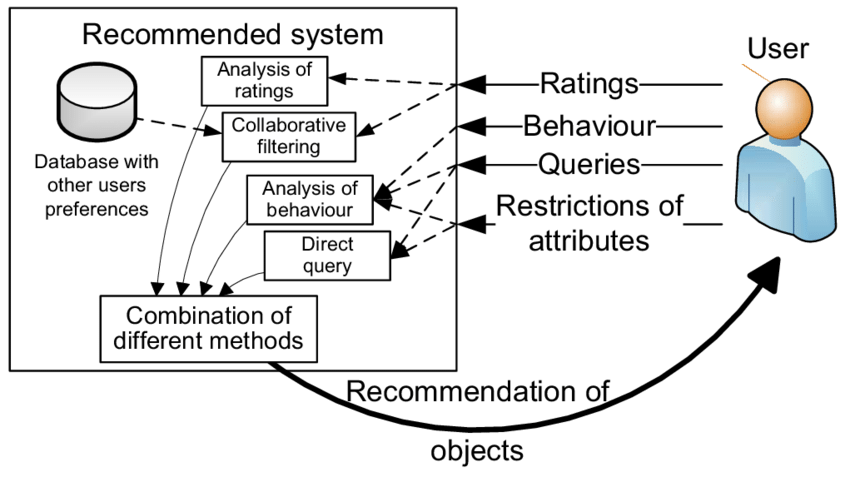
\includegraphics[width=1\textwidth]{algo/algo1.png}
	\end{center}
	\caption{How Recommendation of objects is done ?}
\end{figure}
\linebreak
\lipsum[4]


\subsection{USE CASE DIAGRAM}
\lipsum[4]
\begin{figure}[h!]
	\begin{center}
		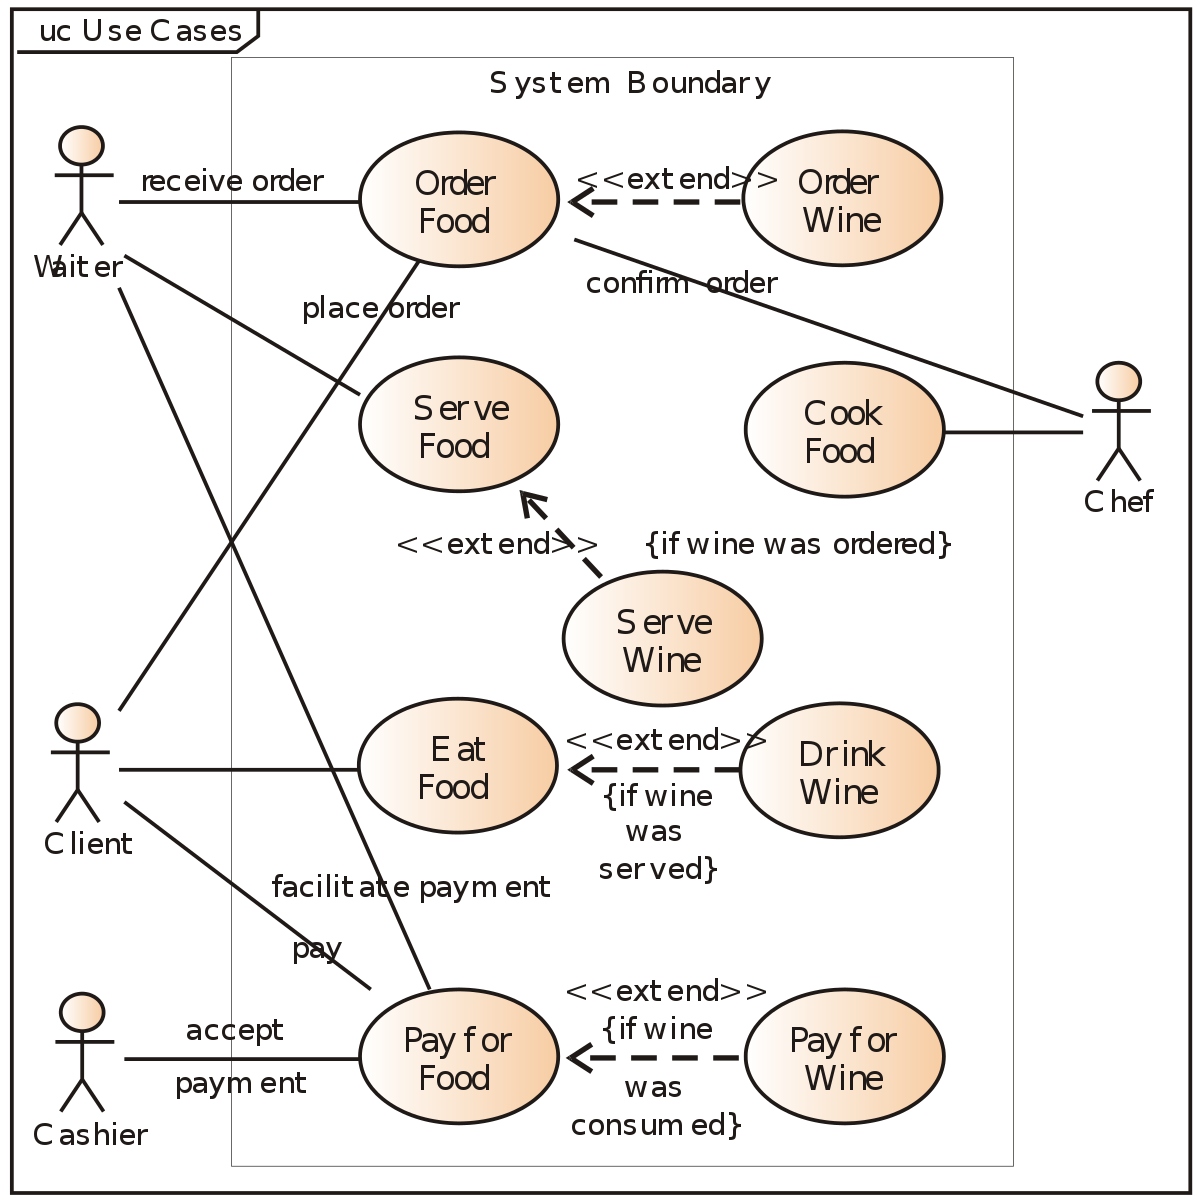
\includegraphics[width=1\textwidth]{uml/usecase.png}
	\end{center}
	\caption{Use case Diagram}
\end{figure}

\subsection{ENTITY RELATIONSHIP DIAGRAM}
\lipsum[4]
\begin{figure}[h!]
	\begin{center}
		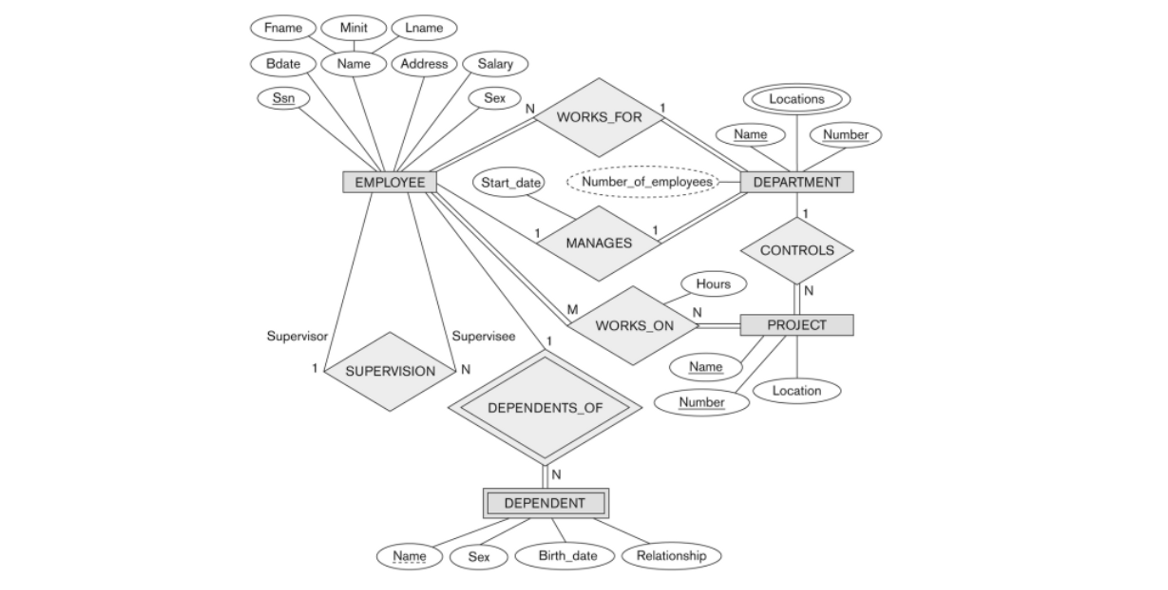
\includegraphics[width=1.3\textwidth]{uml/er.png}
	\end{center}
	\caption{Entity Relationship Diagram}
\end{figure}

\subsection{SYSTEM SEQUENCE DIAGRAM}
\lipsum[4]
\begin{figure}[h!]
	\begin{center}
		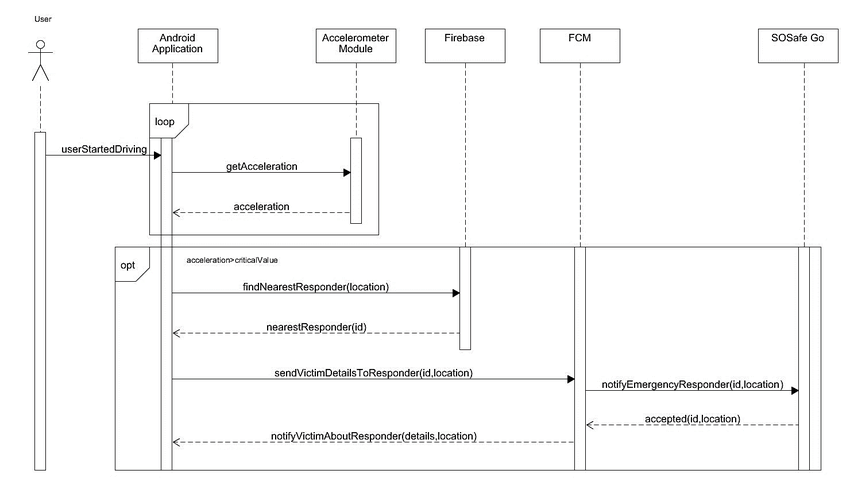
\includegraphics[width=1\textwidth]{uml/ssd.png}
	\end{center}
	\caption{System Sequence Diagram}
\end{figure}

\subsection{CLASS DIAGRAM}
\lipsum[4]
\begin{figure}[h!]
	\begin{center}
		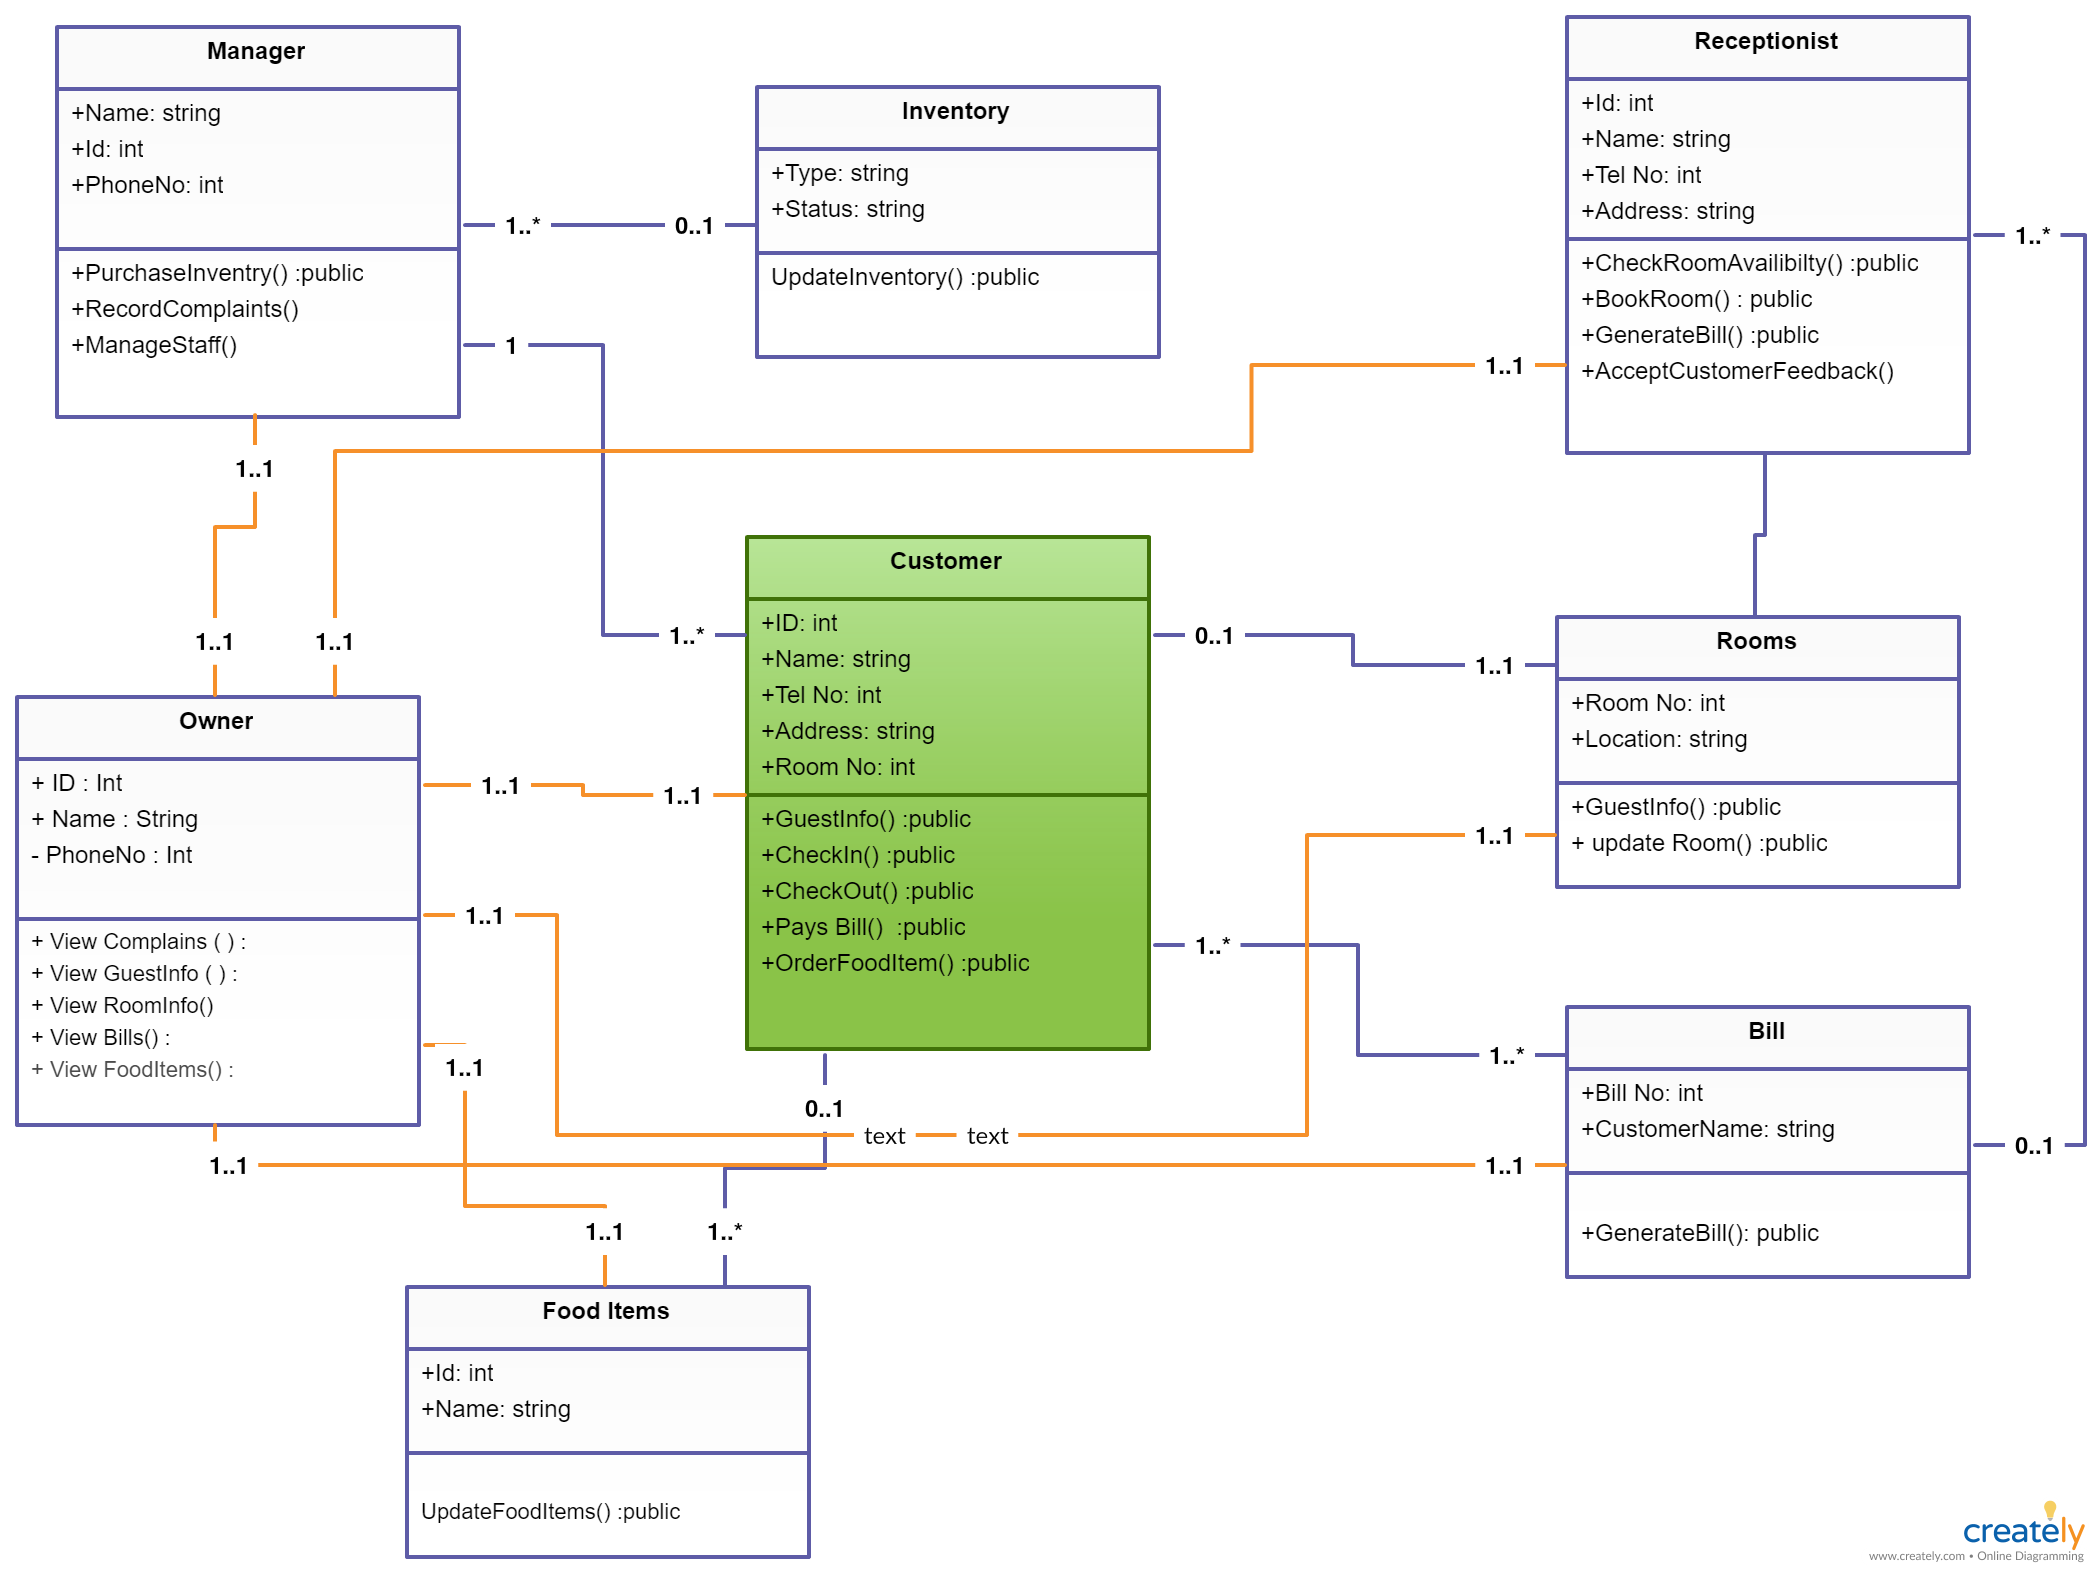
\includegraphics[width=1\textwidth]{uml/class.png}
	\end{center}
	\caption{Class Diagram}
\end{figure}